\section{Background}
\label{sec:background}
Despite recent interest, concerns about system power have existed since the dawn of computing. Some of the earliest valve-based computers had power draws comparable to modern supercomputers. The ENIAC machine dissipated 174 kW \cite{birnbaum:2000aa}, a figure which would not look out of place in the current Top 500 list, despite the fact this machine dates from 1947.\golden

Bipolar semiconductor technologies superseded thermionic valves in the 1950s and 60s, leading to dramatic reduction in power consumption. Over time, manufacturing improvements led to smaller transistors and in turn an exponential increase in both performance and power density. Ultimately this resulted in chips which strained the limits of cooling technologies. \golden

The use of bipolar semiconductors peaked in the early 1990s when they were replaced in turn with the Complementary Metal Oxide Semiconductor (CMOS) technology we still rely on today. CMOS was already mature before this point, however it had been viewed as too slow to be of use in high-performance microprocessors. \golden
\begin{figure}[ht]
\centering
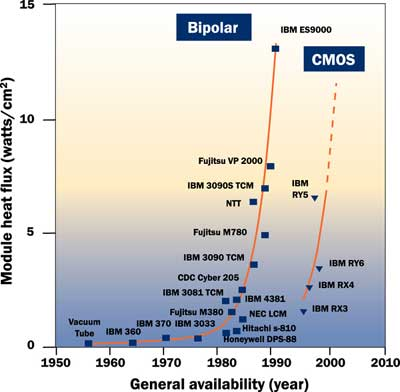
\includegraphics[width=0.9\linewidth]{Images/bipolarcmos.jpg}
\caption{Trends in module level power density, reproduced from \cite{chu:1999aa}. Copyright 1999 IEEE.}
\end{figure}
This pattern of improving hardware until physical limits forces a switch to novel technologies is a recurring one. The previous iteration saw the widespread adoption of multi-core architectures, and once again we find ourselves struggling with the limitations of current hardware. Unfortunately this time we lack a mature semiconductor technology or architectural paradigm waiting in the wings. Researchers are therefore searching for alternative ways to combat the rise of power consumption and ensure continued benefit from technology scaling whilst we await the emergence of the next fundamental shift in processor technology. \golden

System architects are already focussing on power efficient chip design with recent innovations in on-die voltage regulation \cite{burton:2014aa}, Dynamic Voltage and Frequency Scaling (DVFS) scheduling \cite{kwon:2013aa} and \todo{clock gating?}, amongst other areas.

Performance engineers are also looking for ways to address power concerns. It is their efforts we hope to guide with this paper, and hence we constrain our focus to the interaction between software and power consumption for scientific codes. We therefore limit ourselves to considering contemporary CMOS chips with conventional architectures as these make up the majority of supercomputing systems.


The power draw of CMOS chips can be split into distinct components, the most significant of which are dynamic power and leakage power. Dynamic power can be thought of as the power consumed when logic gates change state as a processor performs work. Leakage power dissipation stems from the fact that at very small scales the insulating properties of silicon break down, allowing some current to flow even when gates remain inactive.

\todo{Dennard scaling here. Should cover why pLeak is going to dominate pDyn}



\begin{equation}
\label{eq:totpwr}
P_{tot} = P_{dyn} + P_{leak} + P_{other}
\end{equation}
\begin{equation} 
\label{eq:dynpwr}
P_{dyn} \propto CV^{2}Af
\end{equation}
\begin{equation}
\label{eq:leakpwr}
P_{leak} \propto V\left(ke^{\frac{-qV_{th}}{ak_{a}T}}\right)
\end{equation}

 Equation~\ref{eq:dynpwr} \todo{finish}
here C denotes load capacitance, V the supply voltage, A the activity factor and f the clock frequency.


\fragment{ Dynamic power has traditionally been the dominant source of power consumption}



\fragment{W}



\todo { Find pmbs paper, how they segue into equations}







 We specifically focus on processors from the

\todo{Before we can reduce software power consumption, we must understand its sources and how we measure it}
\todo{The power equations}
\todo{tdp tdp squared etc}
\todo{Linking paragraph, saying now we have metrics we can hope to improve on them}

\todo{Any non-trivial optimization requires tooling support, and that's where we'll head. Say something like the amount we can hope to optimize by is bounded by the size of inefficiency we can detect, because it is fanciful to think we can fix problems we can't see.} 

Code optimisation is a complex task during which developers typically rely on the support of a range tools and techniques including profilers and performance models. Up until now the overarching goal of performance engineers has been to minimize run time. The tools which have emerged over the years have therefore focussed on a specific class of optimization - namely code transformations which speed up execution. An expanded tool set will be required if the kind of multi-objective optimization necessary to encompass both power and runtime is to become commonplace.

A body of research is accumulating as the search for techniques to identify and reason about software power optimizations continues.
\todo{Paragraph stating that work has commenced building up techniques to do this. Note a lot will be covered in prior art.

\begin{itemize}
\item Measurement vs modelling
\item Power is the integral and hard to measure
\end{itemize}
}